\section{Amplificatori Operazionali Reali - 24.09.2014}

In questa esperienza analizzeremo le principali caratteristiche che distinguono un amplificatore operazionale \si{\micro}A741 reale dal suo modello ideale.
In particolare andremo a studiare la tensione di offset e le correnti di polarizzazione - o \textit{bias currents} - cercando di stimare un valore per entrambe, tramite circuiti progettati ad hoc.

Prima di tutto, osserviamo che la circuiteria di alimentazione dell'opamp è la medesima della precedente esperienza e pertanto essa sarà nascosta negli schemi per facilitarne la comprensione.

\subsection*{Strumenti e materiali}

\begin{itemize} [noitemsep]
\item Generatore di tensione continua Agilent E3631A (max $\pm \, \SI{25}{\volt}$ o $\pm \, \SI{6}{\volt}$);
\item Multimetro Agilent 34410A a sei cifre e mezza;
\item Un amplificatore operazionale $\mu$A741;
\item Resistenze e capacità di vari valori;
\item un trimmer a un giro da \SI{5}{\kilo\ohm} e uno da \SI{10}{\kilo\ohm};
\item un trimmer multigiro da \SI{10}{\kilo\ohm};
\item Breadboard e cablaggi vari.
\end{itemize}

\subsection{Stima e correzione dell'offset}
\label{par2:offset}

Un opamp ideale possiede una risposta in uscita perfettamente simmetrica rispetto al caso in cui i due terminali invertente e non invertente sono allo stesso potenziale.
In un opamp reale però, a causa dell'impossibilità di costruire transistor BJT con caratteristiche identiche in modo tale che la circuteria interna dell'integrato risulti simmetrica, è verificata l'esistenza di uno sbilanciamento della risposta in uscita.
La tensione di \textit{offset} $V_{os}$ è definita come la differenza di potenziale tra i terminali di entrata necessaria affinché l'uscita dell'opamp sia nulla.

\subsubsection{Configurazione senza retroazione}

La cosa più semplice da fare per osservare questa imperfezione dell'integrato è collegare entrambi i terminali di ingresso a comune (vedi Figura \ref{cir:open_loop}) e osservare grazie al multimetro la tensione in uscita.
Essa sarà data dalla tensione di offset, amplificata dal guadagno a maglia aperta $A_{ol}$ dell'opamp.
Poiché $A_{ol}$ è un valore particolarmente alto, sebbene $V_{os}$ sia relativamente piccola, spesso accade che l'opamp vada in saturazione.

Nel nostro caso l'opamp andava in saturazione negativa (\SI{-12.9}{\volt}).
Da questo dato si possono trarre due considerazioni: la prima è che il circuito si comporta come se la la tensione all'ingresso invertente fosse maggiore di quella all'ingresso non invertente.
La configurazione a maglia aperta non permette però una stima efficace del valore di $V_{os}$.

La seconda osservazione consiste nel fatto che il modulo della tensione in uscita è inferiore a quello dell'alimentazione usata (\SI{\pm15}{\volt}).
Ciò può essere dovuto alla caratteristica dell'integrato di avere il valore di tensione massimo $|V_{out,max}|$ leggermente inferiore a quello di alimentazione oppure al fatto che $V_{os}$ non è sufficiente per far andare il circuito completamente in saturazione.
Altri gruppi di laboratorio hanno infatti ricavato tensioni di molto inferiori alla tensione di alimentazione del circuito ($\lesssim \SI{10}{\volt}$).

\begin{figure}[ht]
        \centering
	\caption{}
        \begin{subfigure}[b]{0.35\textwidth}
                 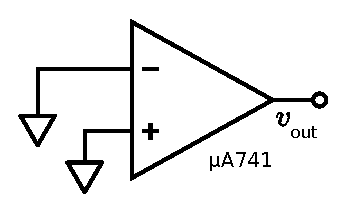
\includegraphics[width=0.70\textwidth]{../E02/latex/open_loop.pdf}
                \caption{Circuito a maglia aperta}
                \label{cir:open_loop}
        \end{subfigure}%
    \quad
        \begin{subfigure}[b]{0.35\textwidth}
               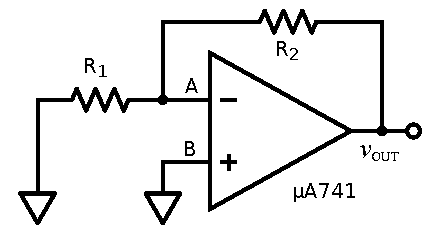
\includegraphics[width=0.70\textwidth]{../E02/latex/inv.pdf}
                \caption{Circuito amplificatore}
                \label{cir:inv}
        \end{subfigure}
\end{figure}

Con il circuito in Figura (\ref{cir:open_loop}) ci è pertanto impossibile ricavare una stima del valore di offset.
Dobbiamo perciò ricorrere a un circuito amplificatore che ci permetta di avere un controllo preciso sul guadagno.

\subsubsection{Configurazione con retroazione}

Lo schema in Figura (\ref{cir:inv}) rappresenta il circuito da noi usato per stimare il valore di $V_{os}$.

Trattiamo per primo il caso del circuito di amplificazione invertente.
L'idea è quella di assumere la presenza di un generatore di tensione che crei una d.d.p. $V_{os}$ tra il terminale invertente e il punto A (l'orientamento del generatore è ininfluente).
In tal modo abbiamo $V_B=0$ e quindi $V_-=V_B=0$, pertanto $V_A = V_{os}$.

Vale allora che, uguagliando le correnti nel nodo A

$$\frac{V_{os}}{R_1} + \frac{V_{os}-V_{out}}{R_2} = 0 \quad \Rightarrow \quad V_{out}=\left(1+\frac{R_2}{R_1}\right) V_{os}$$

Analogamente si tratta il caso non invertente, cioè si assume l'esistenza di un generatore di tensione che crei una d.d.p. $V_{os}$ tra comune (B) e il terminale non invertente.
Anche in questo caso l'orientamento è ininfluente.

Si avrà pertanto $V_B=0$, $V_+=V_{os}$ e pertanto $V_A=V_+=V_{os}$.
L'analisi risulta dunque identica a quella del circuito un amplificatore non invertente, e si ottiene lo stesso risultato del caso invertente, a meno di un fattore $-1$ derivante appunto dall'orientamento del generatore.

Riportiamo nella seguente tabella i valori di offset calcolati, definendo il guadagno come Gain$=1+R_2/R_1$.

\begin{wrapfigure}[17]{l}{0.45\textwidth}
  \caption{Circuito a guadagno unitario. Il trimmer è collegato ai piedini 1 e 5 dell'opamp per compensare l'offset.}
  \begin{center}
  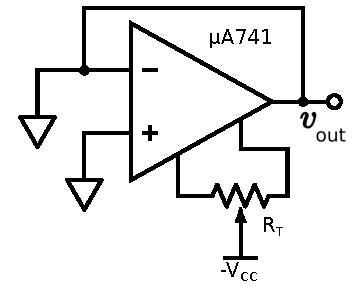
\includegraphics[width=0.30\textwidth]{../E02/latex/trimmer_correction.pdf}
  \end{center}
  \label{cir2:trimmer}
\end{wrapfigure}

\begin{table}[h]
\begin{center}
\begin{savenotes}
\begin{minipage}[c]{0.7\textwidth}
    {\renewcommand{\arraystretch}{1.2}%
	\begin{tabular}{c|c|c|c|c}
		$R_1$ [\si{\ohm}] & $R_2$ [\si{\kilo\ohm}] & Gain &$V_{out}$ [\si{\milli\volt}] & $V_{os}$ [\si{\milli\volt}]\\ 
		\hline 
		$119.8\pm0.1$ & $9.911\pm0.001$ & $83.73\pm0.07$&  $-103.5 \pm 0.5$ & $-1.23 \pm0.01$\\
		\hline
		$119.8\pm0.1$ & $99.35\pm0.01$ & $830.3\pm0.7$ &$ -1025 \pm 2$ & $-1.2 \pm0.1$\\
	\end{tabular}
    }
  \end{minipage}\hfill
  \begin{minipage}[c]{0.3\textwidth}
	\caption{Valori ricavati per la tensione di offset $V_{os}$ con valori nominali per $R_1$ da \SI{120}{\ohm} e per $R_2$ di \SI{10}{\kilo\ohm} e \SI{100}{\kilo\ohm}.}
	\label{tab2:vos}
  \end{minipage}
\end{savenotes}
\end{center}
\end{table}

%Come sappiamo la tensione di offset non è però l'unico problema che incontriamo quando usiamo opamp reali. Infatti ingresso invertente e non invertente sono collegati alle basi di transistor e, ovviamente, per polarizzarli serve una corrente di base. Gli effetti di tale corrente si sommeranno dunque a quelli dovuti all'offset. Tale argomento sarà comunque trattato approfonditamente nella sezione successiva.

Per risolvere il problema della tensione di offset, si può agire collegando una resistenza variabile ai piedini 1 e 5 dell'integrato e all'alimentazione negativa $V^- = \SI{-15}{\volt}$, come mostrato in Figura \ref{cir2:trimmer}.
L'integrato è stato progettato in modo tale che, regolando questa resistenza variabile, data nel nostro caso da un \textit{trimmer resistivo}, si vada a generare una tensione che bilanci l'offset.

Durante l'esperienza abbiamo provato ad utilizzare trimmer resistivo ad un giro da \SI{10}{\kilo\ohm}, ma la sensibilità meccanica del componente era troppo bassa per poter azzerare l'offset: la tensione di uscita infatti passava da saturazione negativa a positiva e viceversa troppo velocemente.

Abbiamo dunque utilizzato un trimmer multigiro da \SI{10}{\kilo\ohm}, con il quale siamo riusciti ad azzerare $V_{out}$.
Togliendo il ramo di retroazione, cioè ponendoci nella situazione di guadagno a maglia aperta, abbiamo misurato la tensione $V_{out}= (1.3\pm0.2)$ \si{\volt}.
Ricordando che $A_{ol} \approx$ 100 - \SI{120}{\decibel}, si nota il buon lavoro svolto sul bilanciamento della tensione di offset.

\begin{wrapfigure}[14]{r}{0.45\textwidth}
  \begin{center}
    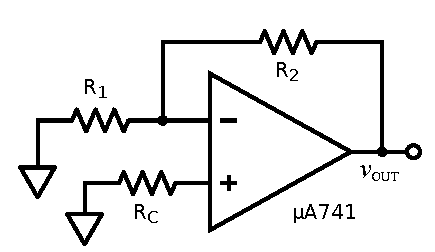
\includegraphics[width=0.310\textwidth]{../E02/latex/current_correction.pdf}
  \end{center}
  \caption{Circuito utilizzato per la stima di $V_{os}$ con la resistenza $R_C$ atta a compensare l'effetto delle correnti di polarizzazione.}
  \label{cir2:current_correction}
\end{wrapfigure}

La tensione di offset non è però l'unico problema da considerare quando usiamo opamp reali.
I terminali invertente e non invertente sono infatti collegati alle basi di due transistor BJT, che per essere polarizzati hanno bisogno di correnti non nulle.
Esse, per quanto piccole, hanno una certa influenza sull'offset totale e maggiore è il valore delle resistenze usate per il circuito di feedback, maggiore è l'effetto di questa corrente sulla stima della tensione di offset.

Per minimizzare questo loro effetto sul valore della tensione di offset, abbiamo posto fra l'ingresso non invertente e comune una resistenza di compensazione $R_C$; il circuito è riportato in Figura \ref{cir2:current_correction}. Il valore di questa resistenza è stato scelto in modo tale da annullare il contributo delle correnti di offset sulla tensione di uscita.

Il contributo sulla tensione di uscita, dato dalle correnti di polarizzazione è:

\begin{equation}
V_{out}^{C} = \left( 1+\frac{R_2}{R_1} \right)\left[ \frac{I_{b^-}R_2}{\frac{R_1+R_2}{R_1}} - I_{b^+} R_B\right]
\label{eq2:Vout_currents}
\end{equation}

supponendo $I_{os} = |I_{b^+}|-|I_{b^-}| \approx 0$ e imponendo $V_{out}^{C}=0$, si ricava che:

$$R_C=\frac{1}{\frac{1}{R_1} + \frac{1}{R_2}} = R_1 // R_2$$

Dai dati riportati in Tabella \ref{tab2:RC} notiamo che le differenze fra i valori della tensione di offset con e senza $R_C$ sono compatibili con il rumore ambientale (qualche decina di \si{\micro\volt} di ampiezza) e pertanto questa misura non è risolutiva.

\begin{table}[H]
\begin{center}
{\renewcommand{\arraystretch}{1.2}%
\begin{tabular}{c|c|c|c|c|c|c}
$R_1$ [\si{\ohm}] & $R_2$ [\si{\kilo\ohm}] & $R_C \approx (R_1 // R_2)$ [\si{\ohm}] & Gain & $V_{out}'$  [\si{\milli\volt}] & $V_{os}'$ [\si{\milli\volt}] & $|V_{os}-V_{os}'|$ [\si{\milli\volt}] \\ 
\hline 
$119.8\pm0.1$ & $9.911\pm0.001$ & $119.4\pm0.1$ & $83.73 \pm 0.07$ & $-105.5 \pm 0.5$ & $-1.26 \pm0.01$ & $0.02\pm0.01$ \\
\hline
$119.8\pm0.1$ & $99.35\pm0.01$ & $119.4\pm0.1$ & $830.3\pm0.7$ &$ -1038 \pm 5$ & $-1.2 \pm 0.1$ & $\approx 0$\\
\end{tabular}}
\end{center}
\caption{Dati ricavati dal circuito con la resistenza $R_C$ collegata tra il terminale non invertente e comune.}
\label{tab2:RC}
\end{table}

\newpage
\subsection{Correnti di polarizzazione}

\begin{wrapfigure}[14]{r}{0.45\textwidth}
  \begin{center}
    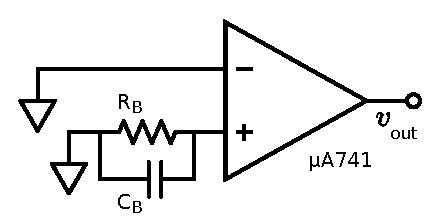
\includegraphics[width=0.320\textwidth]{../E02/latex/direct_measure.pdf}
  \end{center}
  \caption{Schema del circuito senza feedback utilizzato per stimare la corrente di polarizzazione. La resistenza utilizzata è $R_B=10.36\pm0.01$\si{\mega\ohm}; la capacità $C_B=102 \pm 1$ \si{\nano\farad}.}
  \label{cir2:correnti_senzaretroazione}
\end{wrapfigure}

Una volta controbilanciata la caratteristica di offset del nostro opamp, abbiamo quindi analizzato il fenomeno delle correnti di polarizzazione mediante diverse modalità.

\subsubsection{Configurazione senza retroazione}

Unn primo possibile modo di misurare il valore delle correnti di polarizzazione consiste in una misura indiretta che sfrutta la legge di Ohm.
Come si può vedere dallo schema riportato in Figura \ref{cir2:correnti_senzaretroazione}, l'idea è quella di misurare tramite il multimetro la differenza di potenziale ai capi di una resistenza posta, in questo caso, tra il terminale non invertente e comune.

Il valore di corrente cercato sarà dunque:

$$V=I_{b^+} R$$

Per ottenere un valore di tensione sufficientemente alto da essere letto dal nostro multimetro, dato che la corrente di polarizzazione è dell'ordine dei \si{\nano\ampere}, abbiamo utilizzato una resistenza molto grande: $R =$ \SI{10}{\mega\ohm}.

Durante la procedura abbiamo inoltre notato che il valore di tensione sul multimetro fluttuava persino sulla prima cifra, rendendo la nostra misurazione puramente qualitativa (valida al massimo l'ordine di grandezza della corrente).
Per ovviare a questo inconveniente, abbiamo aggiunto in parallelo alla resistenza un condensatore. Questo, caricandosi alla stessa d.d.p. dei capi della resistenza, la stabilizzava.
In questo modo abbiamo potuto ottenere un valore meno fluttuante, che si attestava a $V=(-80 \pm 2)$ \si{\milli\volt}, da cui $I_{b^+}=(7.7 \pm 0.2)$ \si{\nano\ampere}.

Con questo semplice metodo abbiamo potuto ottenere una prima stima del valore della corrente.
Di contro si deve considerare che il valore misurato è particolarmente piccolo ($\approx$\si{\milli\volt}) e quindi è facilmente affetto da rumore ambientale e dalla variazione della resistenza in funzione della temperatura, quindi non è un valore affidabile.

\subsubsection*{Rumore termico}

Per scrupolo abbiamo verificato se una possibile fonte di rumore potesse essere il \textit{rumore termico}, o \textit{rumore Johnson}.
Considerando la larghezza di banda del multimetro $\Delta f = \SI{1}{\hertz}$ e siano $k_B = \SI{1.38e-23}{\joule\per\kelvin}$ la costante di Boltzmann, $T \approx \SI{300}{\kelvin}$ la temperatura assoluta e $R \simeq \SI{10}{\mega\ohm}$ il valore della resistenza presa in considerazione, si ottiene
\begin{equation}
	V_{eff}^2 = 4 k_B T R \Delta f \quad \Rightarrow \quad V_{eff} = \sqrt{4 k_B T R \Delta f} \simeq 4 \times 10^{-7} \si{\volt}
\end{equation}

da cui, ovviamente, si ottiene che il possibile rumore termico è 5 ordini di grandezza inferiore della tensione misurata ed è pertanto ininfluente.
Dunque il rumore presente è sicuramente imputabile ad altre cause probabilmente di tipo ambientale.

\subsubsection{Configurazione con retroazione negativa}

Per ricavare un valore delle correnti di polarizzazione più affidabile abbiamo sfruttato un circuito simile a quello utilizzato per trovare la tensione di offset; lo schema circuitale è mostrato in Figura \ref{cir2:correnti_retroazione_inv}.
Grazie alle proprietà di amplificazione dell'opamp, possiamo ottenere una misura indiretta della corrente di polarizzazione, misurando la tensione in uscita.

\subsubsection*{Misura di $I_{b^-}$}

\begin{wrapfigure}[15]{l}{0.45\textwidth}
  \begin{center}
    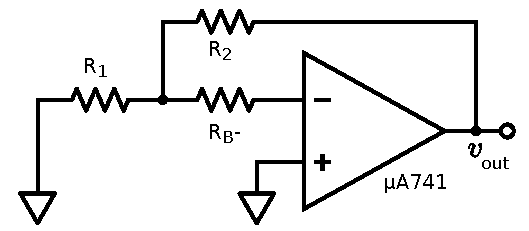
\includegraphics[width=0.330\textwidth]{../E02/latex/inv_current.pdf}
  \end{center}
  \caption{Schema del circuito con feedback utilizzato per stimare la corrente di polarizzazione $I_{b^-}$. Le resistenze utilizzate sono $R_1=(98.9\pm0.1)$ \si{\ohm}, $R_2=(99.4\pm0.1)$ \si{\kilo\ohm} e $R_B=(99.4\pm0.1)$ \si{\kilo\ohm}.}
  \label{cir2:correnti_retroazione_inv}
\end{wrapfigure}

Per risolvere il circuito è sufficiente analizzare la corrente nel nodo in comune alle tre resistenze del circuito $R_1$, $R_2$ e $R_B$.
Considerando $V_-$ la tensione al terminale invertente e $V^*$ la tensione nel nodo analizzato, si ottiene

\begin{equation}
\frac{V^* - 0}{R_1} + \frac{V^*-V_{out}}{R_2} + \frac{V^*-V_{-}}{R_B}=0
\label{eq2:boh}
\end{equation}

Inoltre, dato che la risposta in uscita dell'opamp è stata già bilanciata, possiamo considerare uguali le tensioni agli ingressi invertente e non invertente $V_- = V_+ = \SI{0}{\volt}$.
Da $V^* = R_B I_{b^-}$ e da (\ref{eq2:boh}), con alcuni passaggi algebrici, si ricava che la corrente di polarizzazione $I_{b^-}$ in funzione della tensione di uscita è:

\begin{equation}
I_{b^-}=\frac{V_{out}}{R_2 R_B}\frac{1}{\frac{1}{R_1}+\frac{1}{R_2}+\frac{1}{R_B}}
\label{eq2:boh2}
\end{equation}

Tenendo bene in mente l'equazione \ref{eq2:boh}, le resistenze sono state dimensionate in funzione dell'ordine di grandezza della corrente da misurare.
Considerando il risultato ottenuto precedentemente, volevamo che $V_{out}$ fosse almeno $10^7\approx10^8$ volte più grande della corrente, in modo da utilizzare facilmente il multimetro.
I valori delle resistenze utilizzate sono $R_1=(98.9\pm0.1)$ \si{\ohm}, $R_2=(99.4\pm0.1)$ \si{\kilo\ohm} e $R_B=(99.4\pm0.1)$ \si{\kilo\ohm}.

La misura di tensione in uscita è $V_{out} = (3.89\pm0.02)$ \si{\volt} ed il valore ottenuto per la corrente di polarizzazione del terminale invertente è dunque $I_{b^-} = (38 \pm 5)$ \si{\nano\ampere}.

\subsubsection*{Misura di $I_{b^+}$}

\begin{wrapfigure}[17]{r}{0.45\textwidth}
  \begin{center}
    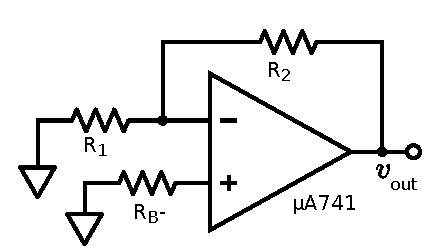
\includegraphics[width=0.3\textwidth]{../E02/latex/ninv_current.pdf}
  \end{center}
  \caption{Schema del circuito con feedback utilizzato per stimare la corrente di polarizzazione $I_{b^+}$. Le resistenze utilizzate sono le medesime del circuito precedente in Figura \ref{cir2:correnti_retroazione_inv}.}
  \label{cir2:correnti_retroazione_noninv}
\end{wrapfigure}

Per misurare la corrente di polarizzazione $I_{b^+}$ abbiamo sfruttato nuovamente il guadagno di un circuito amplificatore con feedback negativo, inserendo però una resistenza $R_B$ tra il terminale non invertente e comune.
Così facendo, il potenziale del terminale non invertente risulta essere $V_+ = I_{b^+} R_B \not= 0$.

Similmente a quanto visto per la configurazione precedente, si analizza il circuito tramite le \textit{regole d'oro} e le leggi di Kirchhoff, ricavando:

$$\frac{V_- - 0}{R_1} + \frac{V_- - V_{out}}{R_2}=0$$

e considerando $V_- = V_+ = I_{b^+} R_B$, otteniamo

\begin{equation}
I_{b^+}=\frac{V_{out}}{R_2 R_B}\frac{1}{\frac{1}{R_1}+\frac{1}{R_2}}
\label{eq2:corrente_noninv}
\end{equation}

Le resistenze sono state dimensionate come per la configurazione precedente e pertanto i valori scelti sono gli stessi riportati in Figura \ref{cir2:correnti_retroazione_noninv}.
La misura di tensione di uscita è $V_{out} = -(3.72 \pm 0.02)$ \si{\volt} ed il valore ottenuto è dunque $I_{b^+} = - (37.2 \pm 0.2)$ \si{\nano\ampere} \footnote{Le correnti di polarizzazione sono in genere scelte entranti nell'opamp. Il valore negativo ricavato per $I_{b^+}$ è quindi da intendersi come una corrente uscente dal terminale non invertente. Al contrario, per il terminale invertente la corrente è intesa entrante poiché il valore di $I_{b^-}$ ha segno positivo.}.

\subsubsection*{Calcolo di $I_{b^+}$ data $I_{b^-}$}

Un altro modo per ricavare il valore della corrente di polarizzazione $I_{b^+}$ è quello di ottenerlo dal valore di $I_{b^-}$, tramite una formula che mette in relazione i due dati.

Osservando il circuito riportato in Figura \ref{cir2:correnti_retroazione_noninv}, si può notare che è identico al circuito in Figura \ref{cir2:current_correction}.
Vale pertanto l'equazione (\ref{eq2:Vout_currents}), da cui è possibile ricavare la dipendenza di $I_{b^+}$ da $I_{b^-}$:

$$I_{b^+} = \frac{R_1}{R_B(R_1+R_2)}(I_{b^-} R_2-V_{out})$$

Inserendo i dati da noi ottenuti ricaviamo $I_{b^+} = - (37.2 \pm 0.2)$ \si{\nano\ampere}, valore compatibile con il risultato del precedente calcolo (eq. (\ref{eq2:corrente_noninv})).

\subsection*{Conclusioni}
In questa esperienza abbiamo potuto osservare come gli opamp, sebbene siano dei circuiti abbastanza precisi, abbiano delle imperfezioni, date dalla loro composizione circuitale (sono presenti dei transistor BJT al loro interno).
Le discrepanze tra il modello ideale e l'opamp reale sono date principalmente dallo sbilanciamento della risposta dello stesso ($V_{os}$) e dalle correnti di polarizzazione (\textit{bias currents}).

Per nostra fortuna spesso gli opamp presentano dei connettori predisposti a minimizzare la tensione di offset con circuiti di compensazione: nel nostro caso un trigger collegato ai piedini di offset e all'alimentazione negativa.
Una volta bilanciato l'opamp, abbiamo misurato le correnti di polarizzazione e abbiamo potuto osservare che esse sono dell'ordine dei \si{\nano\ampere}, quindi trascurabili per gli utilizzi più comuni.
